
\documentclass[journal]{IEEEtran}
\usepackage[a5paper, margin=10mm]{geometry}
%\usepackage{lmodern} % Ensure lmodern is loaded for pdflatex
\usepackage{tfrupee} % Include tfrupee package


\setlength{\headheight}{1cm} % Set the height of the header box
\setlength{\headsep}{0mm}     % Set the distance between the header box and the top of the text


%\usepackage[a5paper, top=10mm, bottom=10mm, left=10mm, right=10mm]{geometry}

%
\setlength{\intextsep}{10pt} % Space between text and floats

\makeindex


\usepackage{cite}
\usepackage{amsmath,amssymb,amsfonts,amsthm}
\usepackage{algorithmic}
\usepackage{graphicx}
\usepackage{textcomp}
\usepackage{xcolor}
\usepackage{txfonts}
\usepackage{listings}
\usepackage{enumitem}
\usepackage{mathtools}
\usepackage{gensymb}
\usepackage{comment}
\usepackage[breaklinks=true]{hyperref}
\usepackage{tkz-euclide} 
\usepackage{listings}
\usepackage{multicol}
\usepackage{xparse}
\usepackage{gvv}
%\def\inputGnumericTable{}                                 
\usepackage[latin1]{inputenc}                                
\usepackage{color}                                            
\usepackage{array}                                            
\usepackage{longtable}                                       
\usepackage{calc}                                             
\usepackage{multirow}                                         
\usepackage{hhline}                                           
\usepackage{ifthen}                                               
\usepackage{lscape}
\usepackage{tabularx}
\usepackage{array}
\usepackage{float}
\usepackage{ar}
\usepackage[version=4]{mhchem}


\newtheorem{theorem}{Theorem}[section]
\newtheorem{problem}{Problem}
\newtheorem{proposition}{Proposition}[section]
\newtheorem{lemma}{Lemma}[section]
\newtheorem{corollary}[theorem]{Corollary}
\newtheorem{example}{Example}[section]
\newtheorem{definition}[problem]{Definition}
\newcommand{\BEQA}{\begin{eqnarray}}
\newcommand{\EEQA}{\end{eqnarray}}

\theoremstyle{remark}


\begin{document}
\bibliographystyle{IEEEtran}
\onecolumn

\title{2.4.22}
\author{INDHIRESH S- EE25BTECH11027}
\maketitle


\renewcommand{\thefigure}{\theenumi}
\renewcommand{\thetable}{\theenumi}

\textbf{Question}  Find the equation of a plane which bisects perpendicularly the line joining the points $A(2, 3, 4)$ and $B(4, 5, 8)$ at right angles.\\
\textbf{Solution}:\\
Let us solve the given equation theoretically and then verify the solution computationally. \\
Let,
\begin{align}
    \Vec{A}=\myvec{2\\3\\4}\;\;and\;\;\Vec{B}=\myvec{4\\5\\8}
\end{align}
Given that the plane is a perpendicular bisector to the line joining points A and B. Since it is a perpendicular bisector to the line joining points A and B , the midpoint of the line joining points A and B lies on the plane.\\
Let the midpoint of points \textbf{A} and \textbf{B} be \textbf{X}. Then
\begin{align}
||\Vec{X}-\Vec{A}||^2=||\Vec{X}-\Vec{B}||^2
\end{align}
\begin{align}
    ||\Vec{X}||^2+||\Vec{A}||^2-2||\Vec{X}||\;||\Vec{A}||= ||\Vec{X}||^2+||\Vec{B}||^2-2||\Vec{X}||\;||\Vec{B}||
\end{align}
\begin{align}
    ||\Vec{A}||^2-2||\Vec{X}||\;||\Vec{A}||=||\Vec{B}||^2-2||\Vec{X}||\;||\Vec{B}||
\end{align}

\begin{align}
   ||\Vec{A}||^2-||\Vec{B}||^2=2\Vec{X^T}\Vec{A}-2\Vec{X^T}\Vec{B}
\end{align}
\begin{align}
    ||\Vec{A}||^2-||\Vec{B}||^2=2\Vec{X^T}(\Vec{A}-\Vec{B})
\end{align}
which can be written as :
\begin{align}
    ||\Vec{A}||^2-||\Vec{B}||^2=2(\Vec{A}-\Vec{B})^T\Vec{X}
\end{align}
\begin{align}
 (\Vec{A}-\Vec{B})^T\Vec{X}=\frac{||\Vec{A}||^2-||\Vec{B}||^2}{2}
\end{align}
Now,
\begin{align}
    \Vec{A}-\Vec{B}=\myvec{2\\3\\4}-\myvec{4\\5\\8}
\end{align}
\begin{align}
   \Vec{A}-\Vec{B}=\myvec{-2\\-2\\-4}
\end{align}
And
\begin{align}
     ||\Vec{A}||=\sqrt{\Vec{A^T}\Vec{A}}
\end{align}
\begin{align}
    ||\Vec{A}||=\sqrt{2(2)+3(3)+4(4)}
\end{align}
\begin{align}
    ||\Vec{A}||=\sqrt{29}
\end{align}

\begin{align}
     ||\Vec{B}||=\sqrt{\Vec{B^T}\Vec{B}}
\end{align}
\begin{align}
     ||\Vec{B}||=\sqrt{4(4)+5(5)+8(8)}
\end{align}
\begin{align}
    ||\Vec{B}||=\sqrt{105}
\end{align}
Now substituting the respective value in Eq.8:
\begin{align}
	\myvec{-2&-2&-4}\Vec{X}=\frac{29-105}{2}
\end{align}
\begin{align}
	\myvec{1&1&2}\Vec{X}=19
\end{align}
Hence the equation of the plane is given by:
\begin{align}
	\myvec{1&1&2}\Vec{X}=19
\end{align}

From the figure it is clearly verified that the theoretical solution matches with the computational solution.\\
\begin{figure}[h]
    \centering
    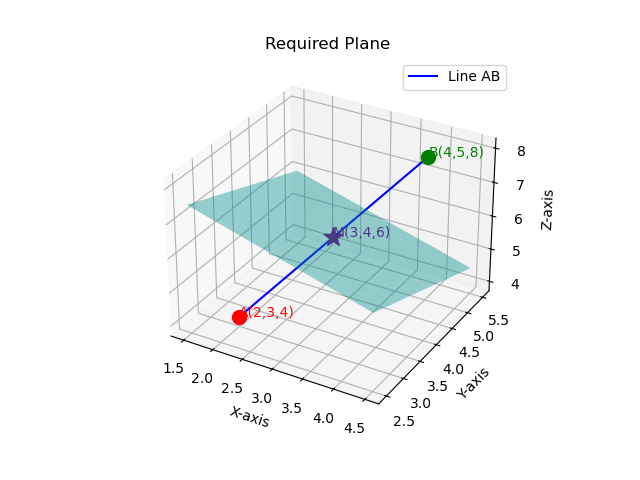
\includegraphics[height=0.5\textheight, keepaspectratio]{figs/figure1.png}
    \label{figure_1}
\end{figure}

\end{document}
\end{document}
